\subsubsubsubsection{Stop}
\begin{figure}[h]
\centering
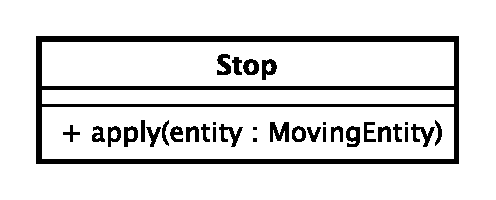
\includegraphics[scale=0.6,keepaspectratio]{images/solution/stop.eps}
\caption{App::Passive::Stop}
\label{fig:sd-app-stop}
\end{figure}
\FloatBarrier
\begin{itemize}
  \item \textbf{Description} \\
It implements the stop road sign. It registers the moving entity for a timeout.
  \item \textbf{Operation}
  \begin{itemize} 
  \item \texttt{+ apply(entity: MovingEntity)} \\
Registers the moving entity for a timeout.
  \end{itemize}
\end{itemize}
